\chapter{Second Example of Grammar Orchestration}
\label{app:example}
To provide a better example of four components in the system, we have created a second example.
$$G_s = (G_1, G_2, G_3, G_4, Q),$$ in which 
\begin{itemize}
    \item{$G_1 = (\{S_1, A, B\},\, \{d_{[-, h, 1, -]}, a_{[-, h, 1, -]}, a_{[-, q, 1, -]},h_{[-, q, 1, -]}, \\ c_{[-, q, 1, -]},a_{[-, q, 1, -]}, f_{[-, q, 1]},f_{[-, h, 1]},e_{[-, q, 1]}\},\, 
    \\ \{1: S_1 \rightarrow (ABAB),
    \\ 2: (A,A) \rightarrow (d_{[-, h, 2]}a_{[-, h, 1]}A, a_{[-, q, 1]}h_{[-, q, 1]}c_{[-, q, 1]}a_{[-, q, 1]}A),
    \\ 3: (A,A) \rightarrow (d_{[-, h, 2]}a_{[-, h, 1]}, a_{[-, q, 1]}h_{[-, q, 1]}c_{[-, q, 1]}a_{[-, q, 1]}),
    \\ 4: (A,A) \rightarrow (f_{[-, q, 1]}e_{[-, q, 1]}f_{[-, h, 1]}A, f_{[-, q, 1]}e_{[-, q, 1]}f_{[-, h, 1]}A),
    \\ 5: (A,A) \rightarrow (f_{[-, q, 1]}e_{[-, q, 1]}f_{[-, h, 1]}, f_{[-, q, 1]}e_{[-, q, 1]}f_{[-, h, 1]}),
    \\ 6: (B,B) \rightarrow (a_{[-, q, 1]}h_{[-, q, 1]}c_{[-, q, 1]}a_{[-, q, 1]}B, d_{[-, h, 2]}a_{[-, h, 1]}B),
    \\ 7: (B,B) \rightarrow (a_{[-, q, 1]}h_{[-, q, 1]}c_{[-, q, 1]}a_{[-, q, 1]}, d_{[-, h, 2]}a_{[-, h, 1]}),
    \})$,}
    \item{$G_2 = (\{S_2, A, B\},\, \{\alpha, \beta, d_{[-, q, 1]}, e_{[-, q, 1]}\},\, 
    \\ \{1: S_2 \rightarrow (ABAB),
    \\ 2: (A,A) \rightarrow (d_{[-, q, 1]}\alpha d_{[-, q, 1]}\alpha A, d_{[-, q, 1]}\alpha d_{[-, q, 1]} \alpha A),
    \\ 3: (A,A) \rightarrow (d_{[-, q, 1]}\alpha d_{[-, q, 1]}\alpha , d_{[-, q, 1]}\alpha d_{[-, q, 1]} \alpha ),
    \\ 4: (B,B) \rightarrow (e_{[-, q, 1]} \beta e_{[-, q, 1]} \beta B, e_{[-, q, 1]} \beta e_{[dim, q, 1]} \beta B),
    \\ 5: (B,B) \rightarrow (e_{[-, q, 1]} \beta e_{[-, q, 1]} \beta , e_{[-, q, 1]} \beta e_{[dim, q, 1]} \beta )
    \})$,}
    \item{$G_3 = (\{S_3, A, B\},\, \{\gamma, \delta, \zeta\},\, 
    \\ \{1: S_3 \rightarrow (ABAB),
    \\ 2: (A,A) \rightarrow (\gamma A, \gamma A),
    \\ 3: (A,A) \rightarrow (\gamma, \gamma),
    \\ 4: (B,B) \rightarrow (\delta B, \delta B),
    \\ 5: (B,B) \rightarrow (\delta, \delta),
    \\ 6: (B,B) \rightarrow (\zeta B, \zeta B),
    \\ 7: (B,B) \rightarrow (\zeta, \zeta)
    \})$,}
    \item{$G_4 = (\{S_4, A, B\},\, \{h_{[-, q, -1]},c_{[-, q, 1]},d_{[-, q, 1]},e_{[-, q, 1]},f_{[-, q, 1]}, g_{[-, q, 1]}, a_{[-, q, 1]},c_{[-, h, 1]}\},\, 
    \\ \{1: S_4 \rightarrow (ABAB),
    \\ 2: (A,A) \rightarrow (c_{[-, q, 1]}e_{[-, q, 1]}g_{[-, q, 1]}e_{[-, q, 1]}A, e_{[-, q, 1]}f_{[-, q, 1]}g_{[-, q, 1]}g_{[-, q, 1]}A),
    \\ 3: (A,A) \rightarrow (c_{[-, q, 1]}e_{[-, q, 1]}g_{[-, q, 1]}e_{[-, q, 1]}, e_{[-, q, 1]}f_{[-, q, 1]}g_{[-, q, 1]}g_{[-, q, 1]}),
    \\ 4: (B,B) \rightarrow (d_{[-, q, 1]}h_{[-, q, -1]}g_{[-, q, 1]}a_{[-, q, 1]}B, h_{[-, q, -1]}d_{[-, q, 1]}c_{[-, h, 1]}B),
    \\ 5: (B,B) \rightarrow (d_{[-, q, 1]}h_{[-, q, -1]}g_{[-, q, 1]}a_{[-, q, 1]}, h_{[-, q, -1]}d_{[-, q, 1]}c_{[-, h, 1]})
    \})$,}
    \item{$Q = \{(1,1,1,1), (2,2,2,2), (3,3,3,3), (4,2,2,2), (5,3,3,3), (6,4,4,4), 
    \\(6,4,6,4), (7,5,7,5)\}$.}
\end{itemize}


\begin{figure}[H]
\centering
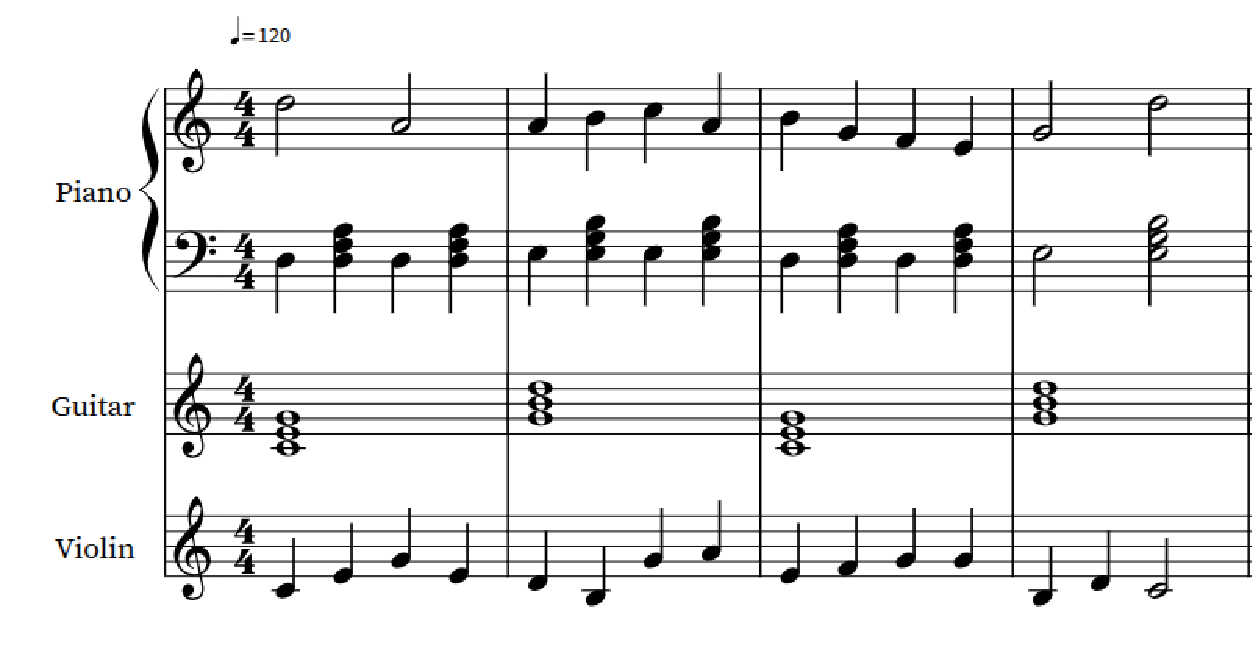
\includegraphics[scale=0.45]{obrazky-figures/Smallexample4.pdf}
\caption{Interpretation of a sentence generated by $G_s$.}
\label{fig:appexample}
\end{figure}

\chapter{Contents of the Storage Medium}
\label{app:content}
Storage medium that stores all the source files for both thesis and implementation has following structure:
\begin{itemize}
    \item{\texttt{src/} - folder contains required source files to run command line application}
    \item{\texttt{thesis/} - folder contains source files that were compiled into \texttt{thesis-makis.pdf}}
    \item{\texttt{thesis-makis.pdf}}
    \item{\texttt{README.md} - files contains installation and setup informations, also there are commands that run the application}
    \item{\texttt{requirements.txt} - required python libraries to run command line application}
\end{itemize}